\documentclass[11pt,compress,t,notes=noshow]{beamer}\usepackage[]{graphicx}\usepackage[]{color}

\makeatletter
\def\maxwidth{ %
  \ifdim\Gin@nat@width>\linewidth
    \linewidth
  \else
    \Gin@nat@width
  \fi
}
\makeatother

\definecolor{fgcolor}{rgb}{0.345, 0.345, 0.345}
\newcommand{\hlnum}[1]{\textcolor[rgb]{0.686,0.059,0.569}{#1}}%
\newcommand{\hlstr}[1]{\textcolor[rgb]{0.192,0.494,0.8}{#1}}%
\newcommand{\hlcom}[1]{\textcolor[rgb]{0.678,0.584,0.686}{\textit{#1}}}%
\newcommand{\hlopt}[1]{\textcolor[rgb]{0,0,0}{#1}}%
\newcommand{\hlstd}[1]{\textcolor[rgb]{0.345,0.345,0.345}{#1}}%
\newcommand{\hlkwa}[1]{\textcolor[rgb]{0.161,0.373,0.58}{\textbf{#1}}}%
\newcommand{\hlkwb}[1]{\textcolor[rgb]{0.69,0.353,0.396}{#1}}%
\newcommand{\hlkwc}[1]{\textcolor[rgb]{0.333,0.667,0.333}{#1}}%
\newcommand{\hlkwd}[1]{\textcolor[rgb]{0.737,0.353,0.396}{\textbf{#1}}}%
\let\hlipl\hlkwb

\usepackage{framed}
\makeatletter
\newenvironment{kframe}{%
 \def\at@end@of@kframe{}%
 \ifinner\ifhmode%
  \def\at@end@of@kframe{\end{minipage}}%
  \begin{minipage}{\columnwidth}%
 \fi\fi%
 \def\FrameCommand##1{\hskip\@totalleftmargin \hskip-\fboxsep
 \colorbox{shadecolor}{##1}\hskip-\fboxsep
     \hskip-\linewidth \hskip-\@totalleftmargin \hskip\columnwidth}%
 \MakeFramed {\advance\hsize-\width
   \@totalleftmargin\z@ \linewidth\hsize
   \@setminipage}}%
 {\par\unskip\endMakeFramed%
 \at@end@of@kframe}
\makeatother

\definecolor{shadecolor}{rgb}{.97, .97, .97}
\definecolor{messagecolor}{rgb}{0, 0, 0}
\definecolor{warningcolor}{rgb}{1, 0, 1}
\definecolor{errorcolor}{rgb}{1, 0, 0}
\definecolor{code}{rgb}{0.97, 0.96, 1.0}
\newenvironment{knitrout}{}{} % an empty environment to be redefined in TeX

\usepackage{alltt}
\usepackage[utf8]{inputenc}
\usepackage[ngerman]{babel}
\usepackage{dsfont}
\usepackage{verbatim}
\usepackage{amsmath}
\usepackage{amsfonts}
\usepackage{mathtools}
\usepackage{csquotes}
\usepackage{cmbright}
\usepackage{multirow}
\usepackage{longtable}
\usepackage{enumerate}
\usepackage[absolute,overlay]{textpos}
\usepackage{psfrag}
\usepackage{algorithm}
\usepackage{algpseudocode}
\usepackage{eqnarray}
\usepackage{bytefield}
\usepackage{animate}
\usepackage{tikz}
\usetikzlibrary{shapes,matrix,positioning,chains,arrows,shadows,decorations.pathmorphing,fit,backgrounds}
\usepackage{adjustbox}
\usepackage{colortbl}
\usepackage{tabularx} % for tables (incl. \hline)
\usepackage{arydshln} % Load after array, longtable, colortab and/or colortbl , otherwise problems with \hline in tabular env
\usepackage{etex} %increase registers for \dimenS to more than 256, otherwise we get "No room for a new \dimen"
\usepackage{graphicx}
\usepackage{booktabs} %used in epr lectures
\usepackage{bm} % bold greek letters
\usepackage{hyperref} % url citing
\usepackage{blkarray} % block arrays
\usepackage{listings} % block of code
\usepackage{xcolor} %colored math symbols
\usepackage{pgffor}
\usepackage{verbatimbox}
\usepackage{xcolor}

%some colors
\definecolor{checkgreen}{HTML}{18A126}
\definecolor{errorred}{HTML}{FF0000}
\definecolor{blockbg}{HTML}{F7F7F7}
\definecolor{gray}{HTML}{A0A0A0}

% basic latex stuff
\newcommand{\col}{\par\colorbox{code}{\parbox{\textwidth}{\theverbbox}}\par}
\newcommand{\eg}{e.\,g.\xspace} %for example
\newcommand{\ie}{i.\,e.\xspace} %that is to say...
\newcommand{\pkg}[1]{{\fontseries{b}\selectfont #1}} %fontstyle for R packages
\newcommand{\lz}{\vspace{0.5cm}} %vertical space
\newcommand{\oneliner}[1] % Oneliner for important statements
{\begin{block}{}\begin{center}\begin{Large}#1\end{Large}\end{center}\end{block}}
\def\SpAr{\quad \Rightarrow \quad}

%new environments
\newenvironment{vbframe}  %frame with breaks and verbatim
{
 \begin{frame}[containsverbatim,allowframebreaks]
}
{
\end{frame}
}

\newenvironment{vframe}  %frame with verbatim without breaks (to avoid numbering one slided frames)
{
 \begin{frame}[containsverbatim]
}
{
\end{frame}
}

\newenvironment{blocki}[1]   % itemize block
{
 \begin{block}{#1}\begin{itemize}
}
{
\end{itemize}\end{block}
}

\newenvironment{fragileframe}[2]{  %fragile frame with framebreaks
\begin{frame}[allowframebreaks, fragile, environment = fragileframe]
\frametitle{#1}
#2}
{\end{frame}}

\newcommand{\myframe}[2]{  %short for frame with framebreaks
\begin{frame}[allowframebreaks]
\frametitle{#1}
#2
\end{frame}}

\usepackage{../../style/lmu-lecture}

\let\code=\texttt
\let\proglang=\textsf

\setkeys{Gin}{width=0.9\textwidth}

\usepackage{tikz}
\usetikzlibrary{shapes,arrows,snakes, calc}

% Define block styles
\tikzstyle{decision} = [diamond, draw, text width=6em, text badly centered, node distance=4cm, inner sep=0pt]
\tikzstyle{decision2} = [diamond, draw, fill=customgreen!35, text width=6em, text badly centered, node distance=4cm, inner sep=0pt]

\tikzstyle{block} = [rectangle, draw, text width=14em, text centered, rounded corners, node distance=3cm, minimum height=4em]
\tikzstyle{line} = [draw, -latex']
\tikzstyle{cloud} = [draw, ellipse, node distance=3cm, minimum height=2em]

\title{Introduction to Deep Learning}
\author{Bernd Bischl}
\institute{Department of Statistics -- LMU Munich}
\date{WS 2021/2022}

\setbeamertemplate{frametitle}{\expandafter\uppercase\expandafter\insertframetitle}

\IfFileExists{upquote.sty}{\usepackage{upquote}}{}
\input{../../latex-math/basic-math}
\input{../../latex-math/basic-ml}
\input{../../latex-math/ml-nn}

\title{Deep Learning}
\date{}

\begin{document}
\newcommand{\titlefigure}{plots/image-compression.png}}
%modify picture
\newcommand{\learninggoals}{
  \item convolutional AEs
  \item applications of AEs 
}



\lecturechapter{Specific Autoencoders and Applications}
\lecture{I2DL}


\begin{vbframe}{Convolutional autoencoder (ConvAE)}
  \begin{itemize}
    \item %n the last example, we have seen that autoencoder inputs are images. So, it makes sense to ask whether a convolutional architecture can work better than the autoencoder architectures discussed previously.
    For the image domain, using convolutions is advantageous. Can we also make use of them in AEs?     
    \item In a ConvAE, the encoder consists of convolutional layers. The decoder, on the other hand, consists of transpose convolution layers or simple upsampling operations.
   % \begin{itemize}
  %    \item Instead of convolving a filter mask with an image, to get a set of activations as in a CNN, we are trying to infer the activations that when convolved with the filter mask, would yield the image.
   % \end{itemize}
   % \item The original aim was to learn a hierarchy of features in an unsupervised manner. However, now its more commonly being used to invert the downsampling that takes place in a convolutional network and \enquote{expand} the image back to its original size.
  \end{itemize}
\framebreak
  \begin{figure}
    \centering
    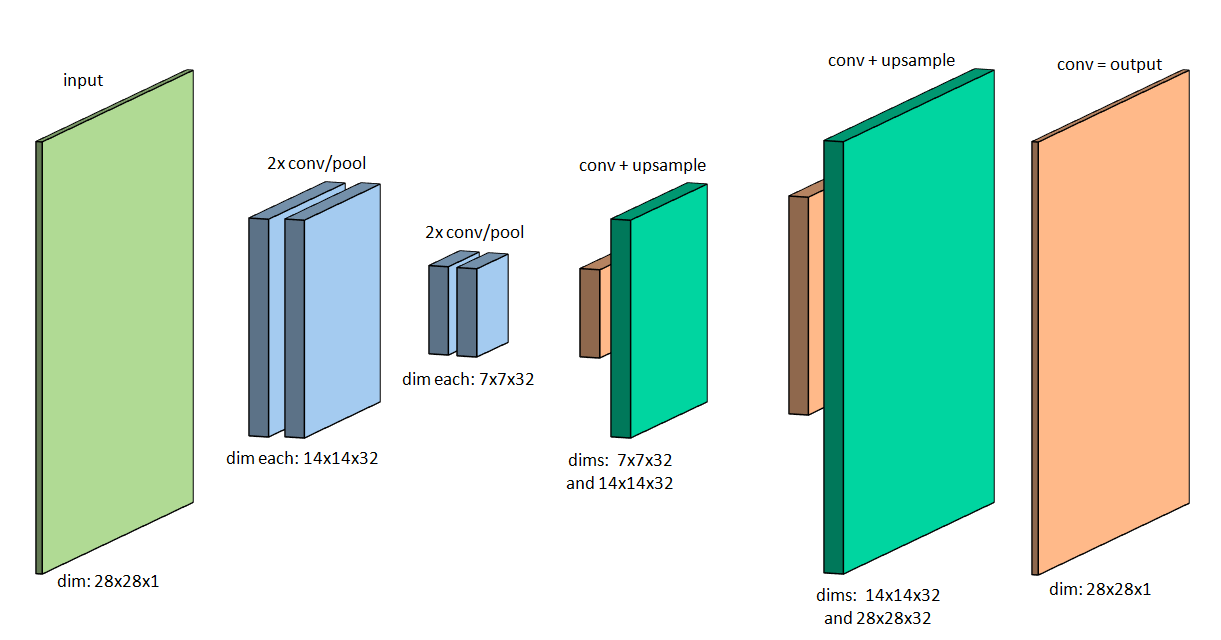
\includegraphics[width=11cm]{plots/convolutional_autoencoder3.png}
    \caption{Potential architecture of a convolutional autoencoder.}
  \end{figure}
  We now apply this architecture to denoise MNIST.
\framebreak
  \begin{figure}
    \centering
    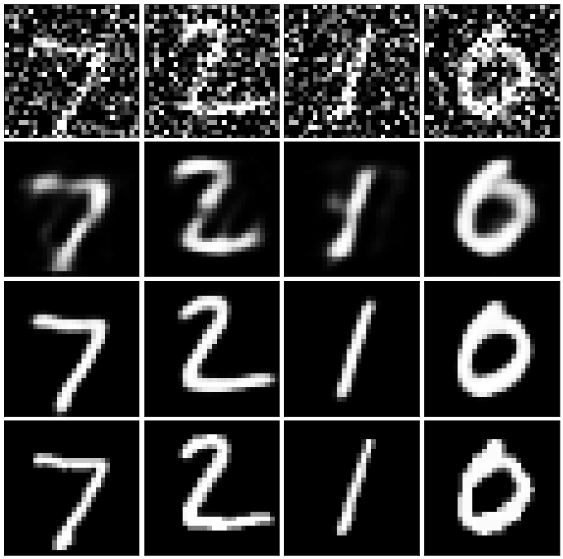
\includegraphics[width=6.3cm]{plots/convolutional_autoencoder2.png}
    \caption{Top row: noised data, second row: AE with $dim(\pmb{z}) = 32$ (roughly 50k params), third row: ConvAE (roughly 25k params), fourth row: ground truth.}
  \end{figure}
%\framebreak
%  Convolutional autoencoders may also be used for image segmentation:
%  \begin{figure}
%    \centering
%    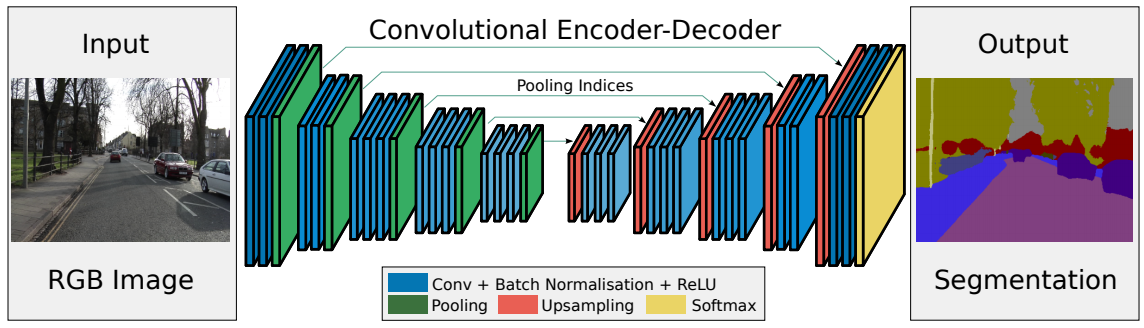
\includegraphics[width=11cm]{plots/convolutional_autoencoder.png}
%    \caption{SegNet: A Deep Convolutional Encoder-Decoder Architecture for Image Segmentation (Vijay Badrinarayanan et al. (2016))}
%  \end{figure}
\end{vbframe}
%%%%%%%%%%%%%%%%%%%%%%%%%%%%%%%%%%%%%%%%%%%%%%%%%%%%%%%%%%%%%%%%%%
%%%%%%%%%%%%%%%%%%%%%%%%%%%%%%%%%%%%%%%%%%%%%%%%%%%%%%%%%%%%%%%%%%
% \begin{vbframe}{AEs for unsupervised pretraining}
%   \begin{itemize}
%     \item Stacked AEs can be used for layer-wise unsupervised pretraining of deep neural networks.
%     \item This corresponds to subsequently training each layer as an AE.  
%     \item It aims  at yielding better weight initializations for the actual supervised training.
%     \item This usually eliminates the risk of vanishing gradients in feed forward nets.
%     \item It played an important role in the past before general techniques for stabilizing optimization were invented (e.g.~ReLUs, batch normalization, dropout, etc.)
%   \end{itemize}
% \end{vbframe}


\begin{vbframe}{Real-world Applications}

Today, autoencoders are still used for tasks such as: 
\begin{itemize}
\item  data de-noising,
\item  compression,
\item and dimensionality reduction for the purpose of visualization.
\end{itemize}

\framebreak 
  \textbf{Medical image denoising} using convolutional denoising autoencoders
  \begin{figure}
    \centering
    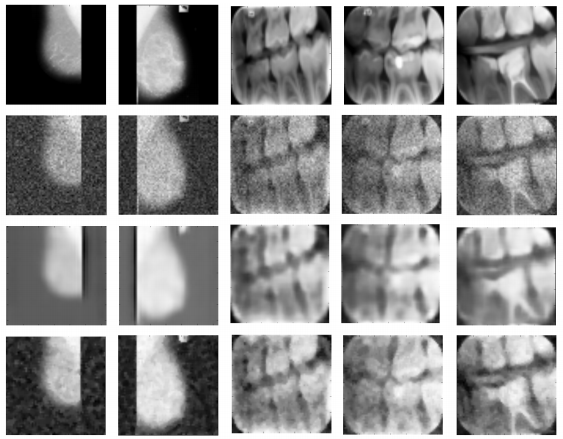
\includegraphics[width=6.5cm]{plots/denoising_autoencoder_application.png}
    \caption{Top row : real image, second row   : noisy version, third row : results of a (convolutional) denoising autoencoder and fourth row : results of a median filter (Lovedeep Gondara (2016))}
  \end{figure}
  
  \framebreak
  AE-based \textbf{image compression}.
  \begin{figure}
    \centering
    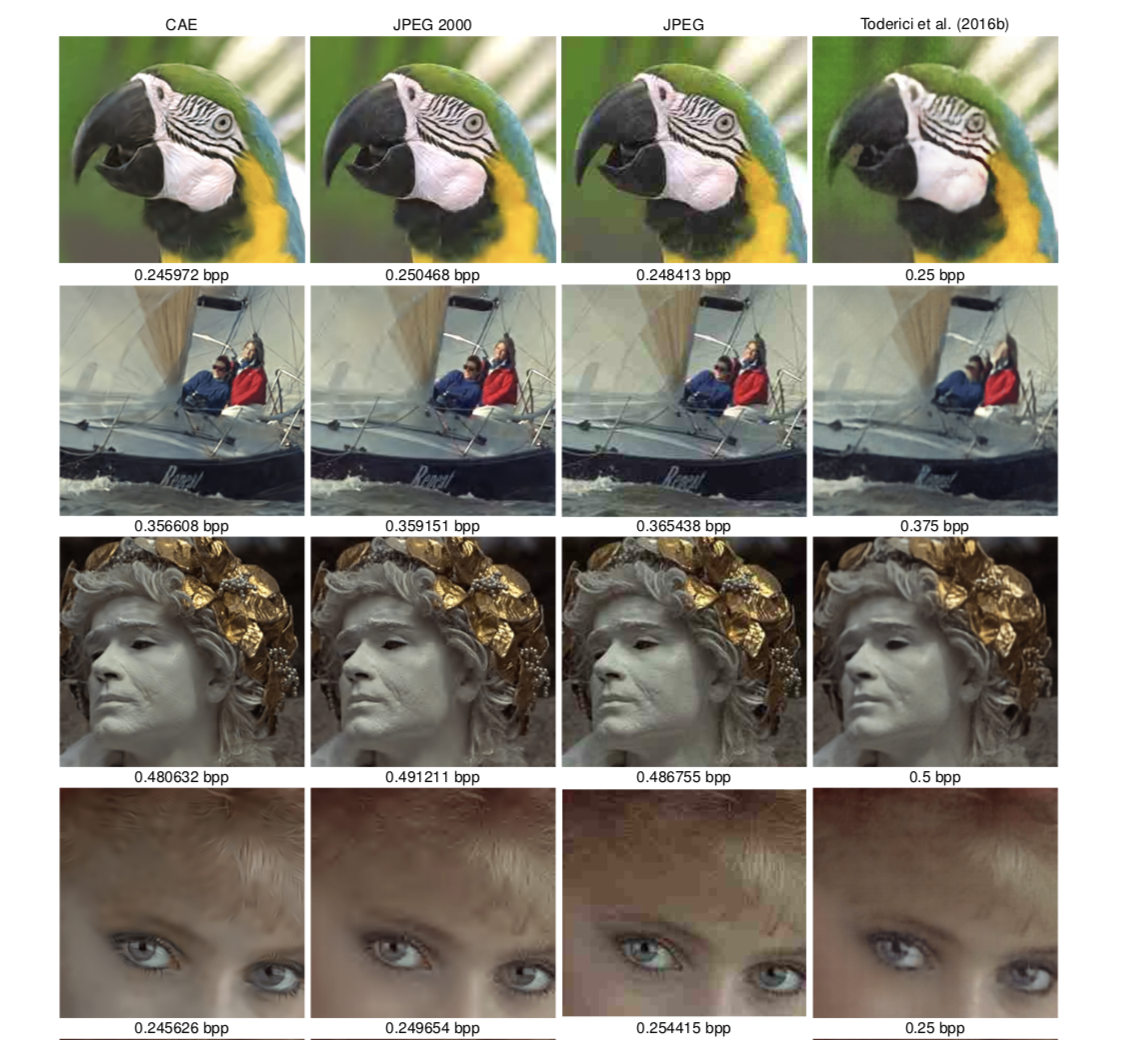
\includegraphics[width=6.5cm]{plots/image-compression.png}
    \caption{from Theis et al. }
    \end{figure}
  
  
\end{vbframe}


\endlecture
\end{document}